\documentclass{beamer}
\usetheme{Copenhagen}
\usecolortheme{seahorse}
\usefonttheme[onlymath]{serif}

\usepackage{setspace}
\usepackage{xcolor}
\usepackage{graphicx}
\usepackage{multimedia}
\usepackage{fontawesome5}
\usepackage[most]{tcolorbox}
\usepackage{empheq}
\usepackage{fancybox}
\usepackage{annotate-equations}
\usepackage{tikz}
\usetikzlibrary{positioning, calc, shapes.geometric, shapes.multipart, 
	shapes, arrows.meta, arrows, 
	decorations.markings, external, trees}
\tikzstyle{Arrow} = [
thick, 
decoration={
	markings,
	mark=at position 1 with {
		\arrow[thick]{latex}
	}
}, 
shorten >= 3pt, preaction = {decorate}
]

\definecolor{teel}{HTML}{00AEB3}
\definecolor{redorange}{HTML}{F26035}
\definecolor{ForestGreen}{RGB}{34,139,34}
\definecolor{darkgreen}{HTML}{06402B}
\definecolor{CarolinaBlue}{HTML}{4B9CD3}
\usecolortheme[named=CarolinaBlue]{structure}

\newenvironment{variableblock}[3]{%
	\setbeamercolor{block body}{#2}
	\setbeamercolor{block title}{#3}
	\begin{block}{#1}}{\end{block}}


\title[Augmented Trials]{Using observational data to improve inference in randomized trials}
\author[Paul Zivich]{Paul Zivich \\~\\ Assistant Professor \\ Department of Epidemiology \\ Gillings School of Global Public Health \\ University of North Carolina at Chapel Hill}

\setbeamercovered{transparent}
\setbeamertemplate{navigation symbols}{}  % gets rid of the dumb navigation symbols
\setbeamertemplate{page number in head/foot}{\insertframenumber}  % adds slide #
\setbeamertemplate{headline}{}

\AtBeginSection[]{
	\begin{frame}
		\vfill
		\centering
		\begin{beamercolorbox}[sep=8pt,center,shadow=true,rounded=true]{title}
			\usebeamerfont{title}\insertsectionhead\par%
		\end{beamercolorbox}
		\vfill
	\end{frame}
}

\begin{document}
	
\begin{frame}[plain]
	\maketitle
\end{frame}

\begin{frame}{Acknowledgements\footnote[frame]{Footnotes are for asides or references, but are fair game for questions}}
	\textbf{Funding}: K01AI177102, P30AI50410, R01AI157758 \\~\\
	\textbf{Disclaimer}: views (and errors) are mine and not those of colleagues, NIH, DHHS, US government \\~\\
	\begin{center}
		\small
		\faEnvelope \quad pzivich@unc.edu \qquad \quad 
		\faGithub \quad pzivich \qquad \quad
		\faHashtag \quad pausalz@bsky.social
	\end{center}
\end{frame}

\begin{frame}{Preventing Vertical HIV Transmission}
	Standard of Care (SOC):
	\begin{itemize}
		\item Maternal antiretroviral (ARV) therapy 
		\item Short-term daily infant ARV prophylaxis
	\end{itemize}
	~\\
	Transmission still occurs
	\begin{itemize}
		\item Postpartum viral rebound \& breastfeeding
		\begin{itemize}
			\item Still recommended because of survival benefits\footnote[frame]{Thior et al. \textit{JAMA} 2006}
		\end{itemize}
	\end{itemize}
	~\\
	Long-acting injectable (LAI) ARV
	\begin{itemize}
		\item Simplified administration
		\item Longer efficacy
	\end{itemize}
\end{frame}

\begin{frame}{Regulatory Approval for LAI-ARV in Infants}
	Challenges
	\begin{itemize}
		\item Extrapolating efficacy from adults unlikely to be acceptable
		\item Need an active-control trial
		\begin{itemize}
			\item Low risk of transmission under standard of care\footnote[frame]{Around 0.6\% in previous trials; Fowler et al. \textit{N Engl J Med} 2016}
		\end{itemize}
		\item Sample sizes difficult to meet, costs
	\end{itemize}
\end{frame}

\begin{frame}{A Solution}
	Augmented Trial Design
	\begin{itemize}
		\item Fuse trial and prospective observational cohort
	\end{itemize}
	~\\
	\begin{center}
		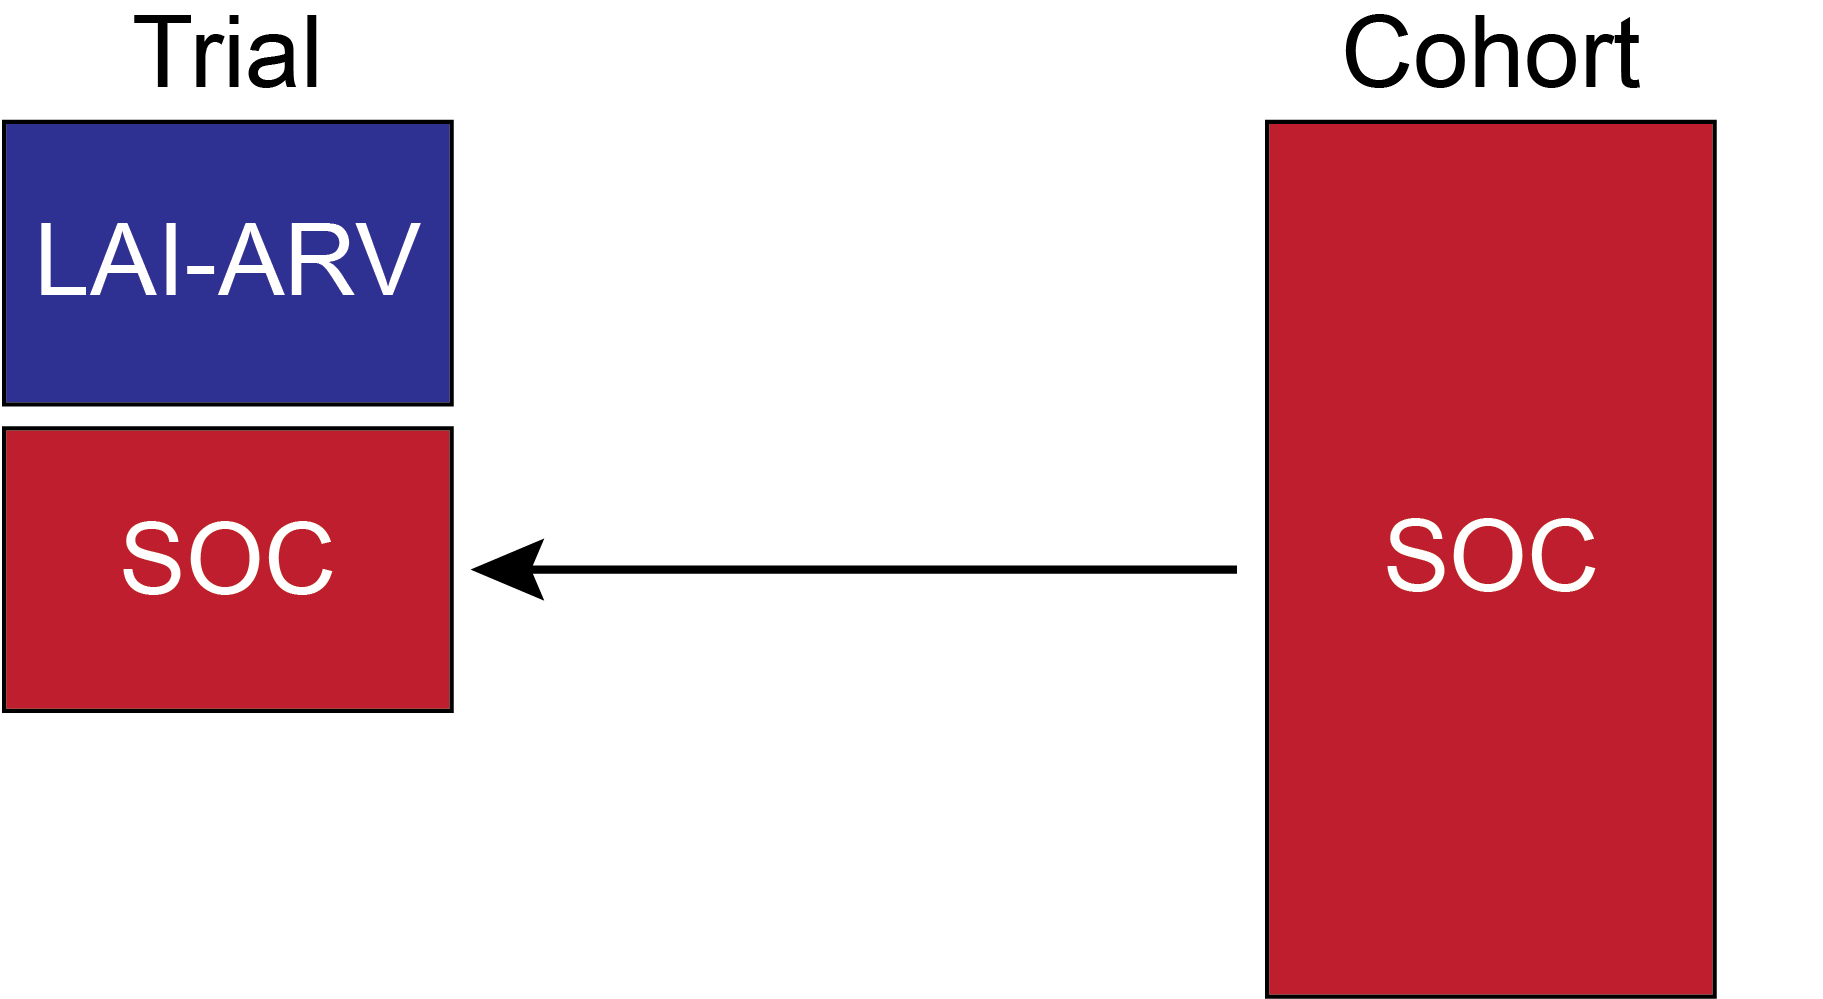
\includegraphics[width=0.8\linewidth]{images/schematic.png}
	\end{center}
\end{frame}

\begin{frame}{Notation}
	$Y^a_i$: potential outcome for unit $i$ under action $a$ \\
	~\\
	$A_i$: action for unit $i$ \\
	$Y_i$: observed outcome for unit $i$ \\
	$S_i$: population indicator ($1$: trial $0$: cohort) \\
	$W_i$: baseline covariate related to $Y$ and (maybe) $S$ \\
	$O_i = (S_i, W_i, A_i, Y_i)$ \\
	~\\
	$f_X(x)$: probability density function at $x$ for variable $X$ \\
	$E[\cdot]$: expected value function \\
	~\\
	$$\tau = \mu_1 - \mu_0 = E[Y^1 \mid S=1] - E[Y^0 \mid S=1]$$
\end{frame}

\begin{frame}{Identification}
	\begin{block}{1: Causal Consistency}
		\begin{equation*}
			Y_i = Y_i^a \text{ if } a=A_i
		\end{equation*}
	\end{block}
	\begin{block}{2.1: Action Exchangeability}
		\begin{equation*}
			Y_i^a \amalg A_i \mid W_i
		\end{equation*}
	\end{block}
	\begin{block}{2.2: Action Positivity}
		\begin{equation*}
			\forall w \in \mathcal{W}\left[ 0 < \Pr(A=1 \mid W=w) < 1 \right] 
		\end{equation*}
	\end{block}
	\begin{variableblock}{3.1: Sampling Exchangeability}{bg=red!20,fg=black}{bg=red!90,fg=white}
		\begin{equation*}
			Y_i^a \amalg S_i \mid W_i
		\end{equation*}
	\end{variableblock}
	\begin{variableblock}{3.2: Sampling Positivity}{bg=red!20,fg=black}{bg=red!90,fg=white}
		\begin{equation*}
			f_{W \mid S=1}(w) > 0 \implies f_{W}(w \mid S=0) > 0
		\end{equation*}
	\end{variableblock}
\end{frame}

\begin{frame}{Estimation}
	Estimating equations are defined as \footnote[frame]{Stefanski \& Boos \textit{Am Stat} 2002; Ross et al. \textit{IJE} 2024}
	~\\~\\~\\~\\
	\begin{equation*}
		\sum_{i=1}^{n}
		\eqnmarkbox[blue]{node1}{
			\eqnmark[blue]{node1a}{\psi}(
			\eqnmark[red]{node1b}{O_i}, 
			\eqnmark[violet]{node1c}{\hat{\theta}}
			)}
		= 0
	\end{equation*}
	\annotate[yshift=2em]{left}{node1a}{Estimating function}	
	\annotate[yshift=-1em]{below,left}{node1b}{Observation $i$}
	\annotate[yshift=1em]{right}{node1c}{Estimated parameters}
\end{frame}

\begin{frame}{Trial-Only Estimator}
	\begin{equation*}
		\psi_{T}(O_i; \theta) = 
		\begin{bmatrix}
			\eqnmarkbox[red]{node0}{S_i (1 - A_i) (Y_i - \mu_0)} \\ 
			\eqnmarkbox[blue]{node1}{S_i A_i (Y_i - \mu_1)} \\ 
			\eqnmarkbox[violet]{node2}{(\mu_1 - \mu_0) - \tau} \\
		\end{bmatrix}
	\end{equation*}
	Only trial observations ($S_i = 1$) contribute information
\end{frame}

\begin{frame}{Fusion Estimator\footnote[frame]{This estimator is consistent as long as either the sampling model or outcome model is correctly specified}}
	\begin{equation*}
		\psi_{F}(O_i; \theta) = 
		\begin{bmatrix}
			\eqnmarkbox[green]{node4}{(S_i - \widehat{S}_i ) \mathbb{W}_i^T} \\
			\eqnmarkbox[orange]{node5}{\pi_{S_i} (1-A_i) (Y_i - \widehat{Y}_i ) \mathbb{X}_i^T} \\
			\eqnmarkbox[red]{node0}{S_i (\widehat{Y}_i - \mu_0)} \\ 
			\eqnmarkbox[blue]{node1}{S_i A_i (Y_i - \mu_1)} \\ 
			\eqnmarkbox[violet]{node2}{(\mu_1 - \mu_0) - \tau} \\
		\end{bmatrix}
	\end{equation*}
	where 
	\begin{itemize}
		\item $\widehat{S}_i = \text{expit}(\mathbb{W}_i \alpha^T)$ and $\mathbb{W}_i$ is a design matrix including $W$
		\item $\pi_{S_i} = S_i + (1-S_i)\frac{\widehat{S}_i}{1-\widehat{S}_i}$
		\item $\widehat{Y}_i = \text{expit}(\mathbb{X}_i \beta^T)$ and $\mathbb{X}_i$ is a design matrix including $W$
	\end{itemize}
\end{frame}

\section{Simulations}

\begin{frame}{Simulation -- Design}
	Trial
	\begin{equation*}
		\begin{bmatrix}
			W \sim \text{Bernoulli}(\eqnmark[blue]{node1}{0.\bar{6}}) \\
			A \sim \text{Bernoulli}(p)
		\end{bmatrix}
	\end{equation*}
	Observational Cohort
	\begin{equation*}
		\begin{bmatrix}
			W \sim \text{Bernoulli}(\eqnmark[red]{node2}{0.2}) \\
			A := 0
		\end{bmatrix}
	\end{equation*}
	Outcome model
	\[ Y \sim \text{Bernoulli}(0.01 + 0.015 W (1-A)) \]
	$$ \tau = 0.01 $$
\end{frame}

\begin{frame}{Simulation -- Design}
	Assess Power at $\alpha = 0.05$ for
	\begin{itemize}
		\item for 1:1 and 3:1 randomization
		\item varying trial and observational cohort sizes
	\end{itemize}
	~\\
	 with 5000 data sets
\end{frame}

\begin{frame}{Simulation -- Power by Trial Size\footnote[frame]{For an observational cohort of 5000}}
	\begin{center}
		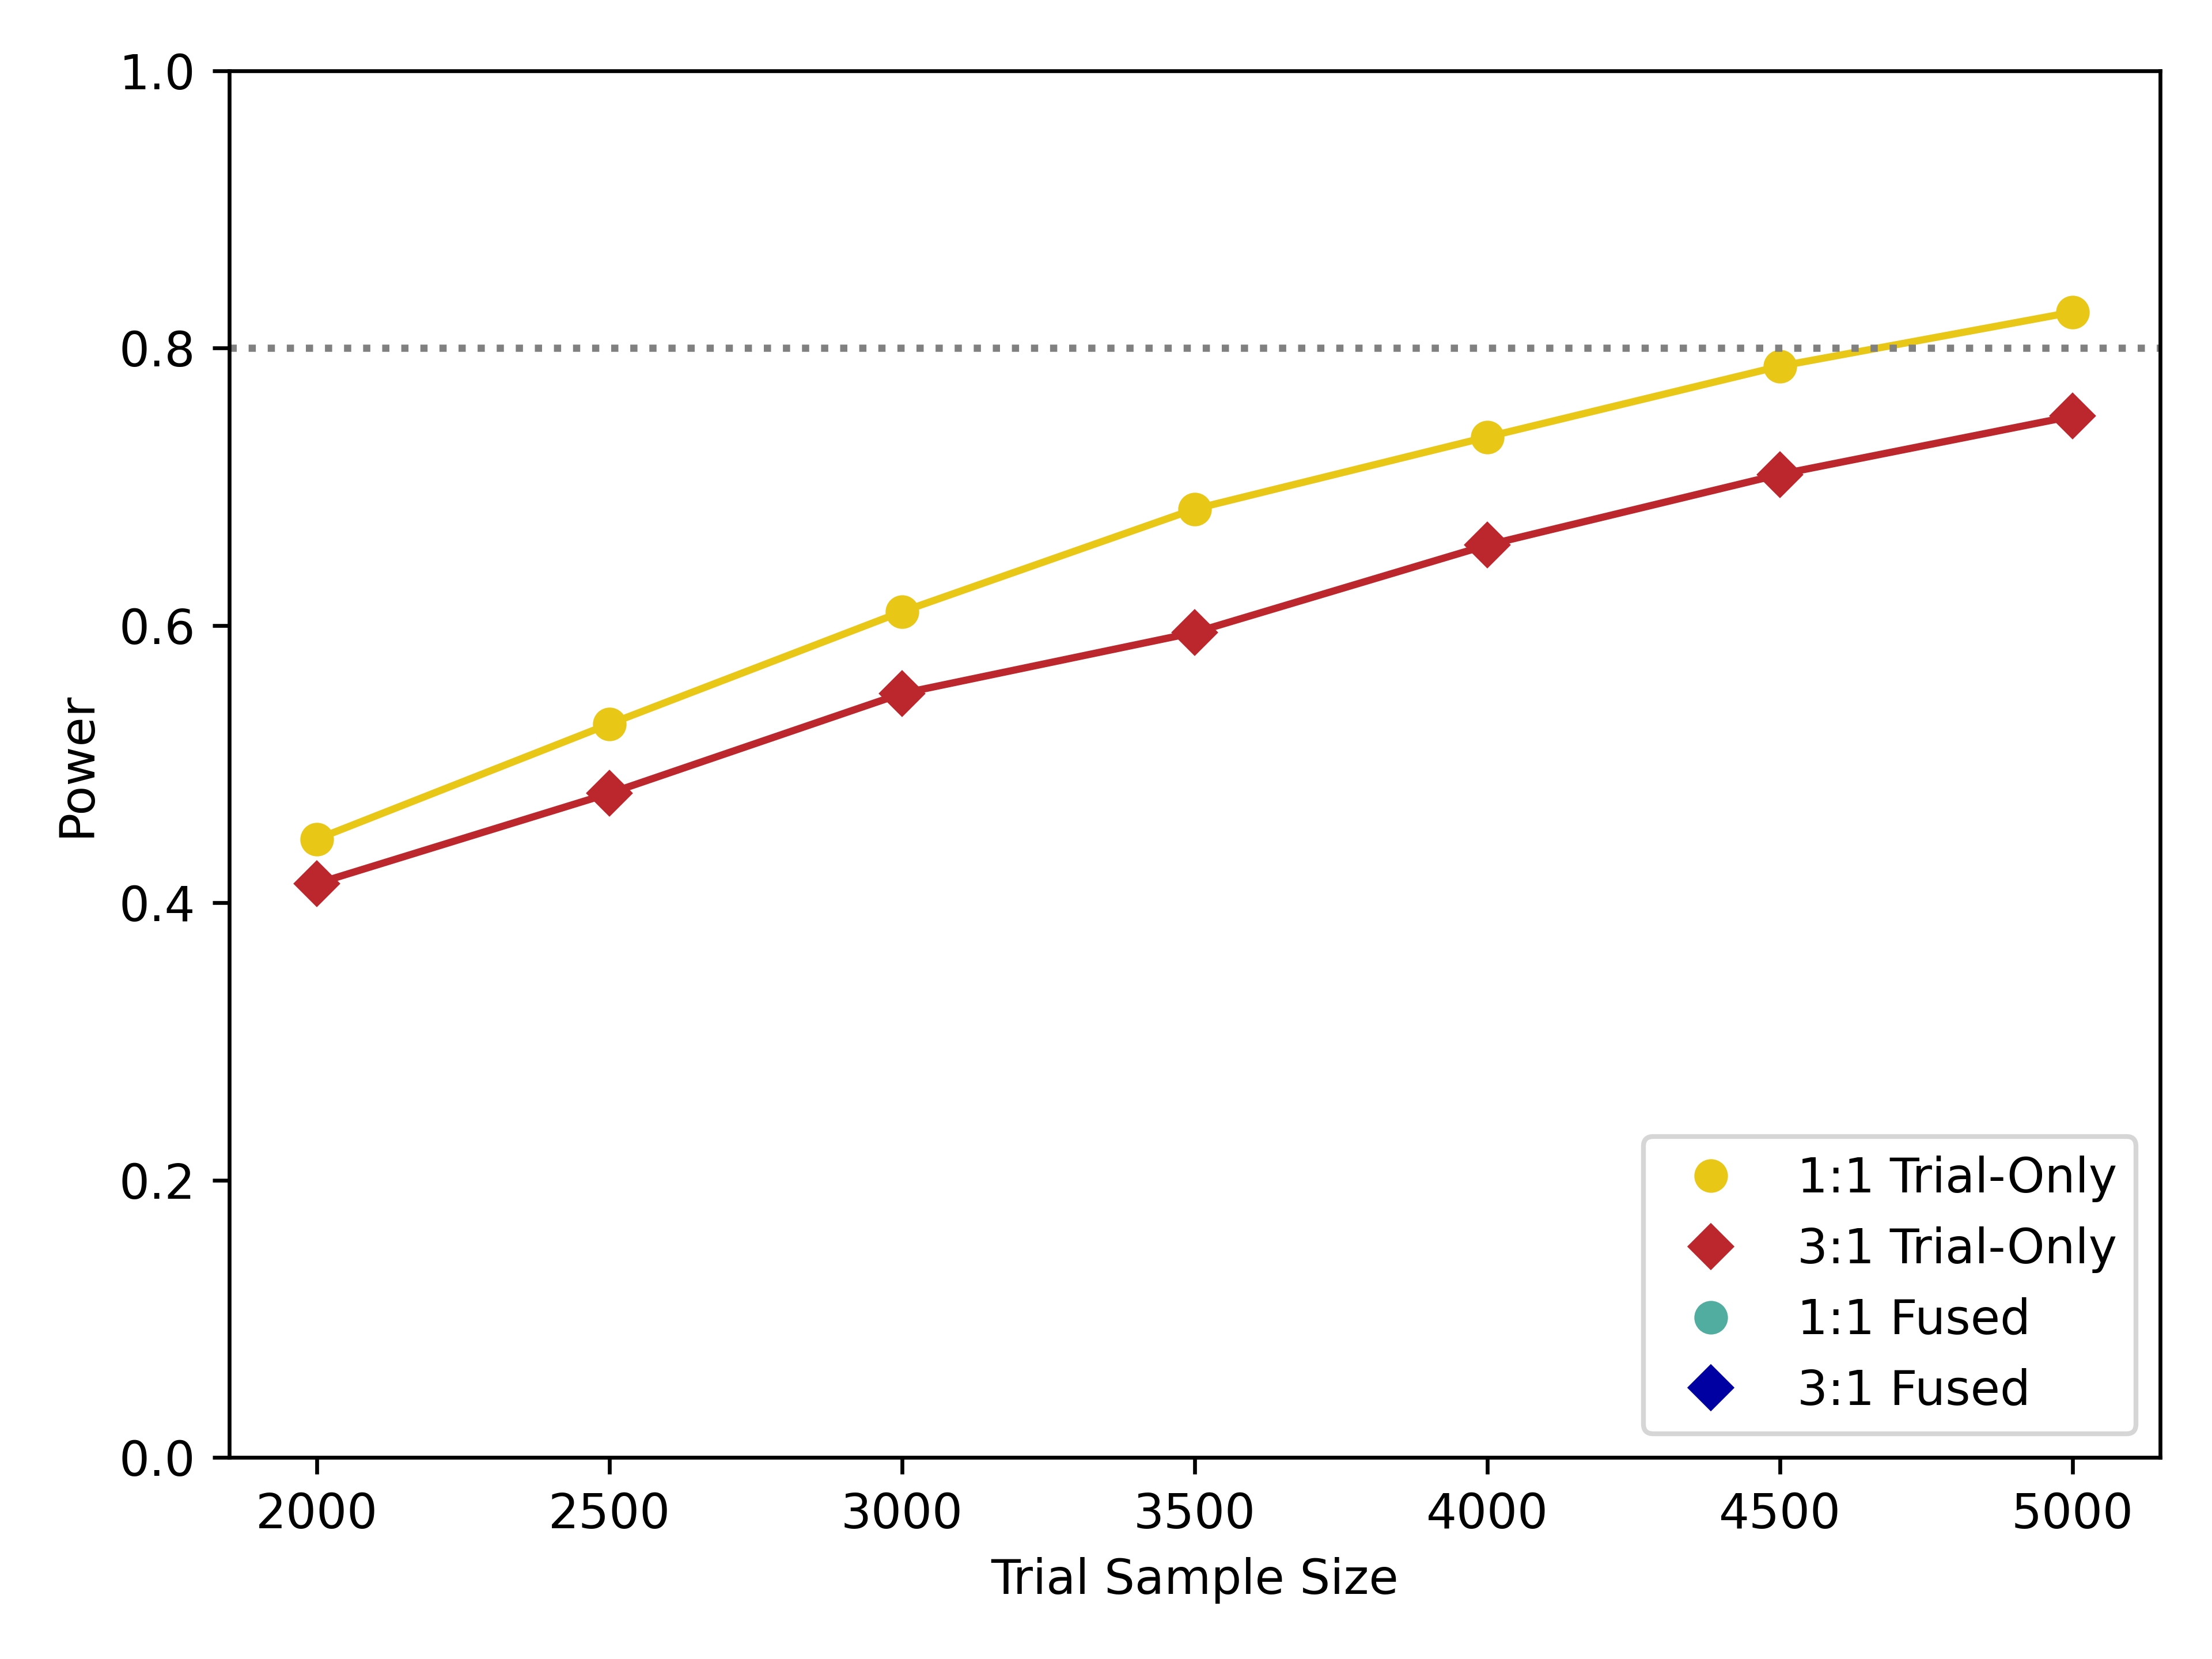
\includegraphics[width=0.9\linewidth]{images/power_trial-n_ser1.png}
	\end{center}
\end{frame}

\begin{frame}{Simulation -- Power by Trial Size\footnote[frame]{For an observational cohort of 5000}}
	\begin{center}
		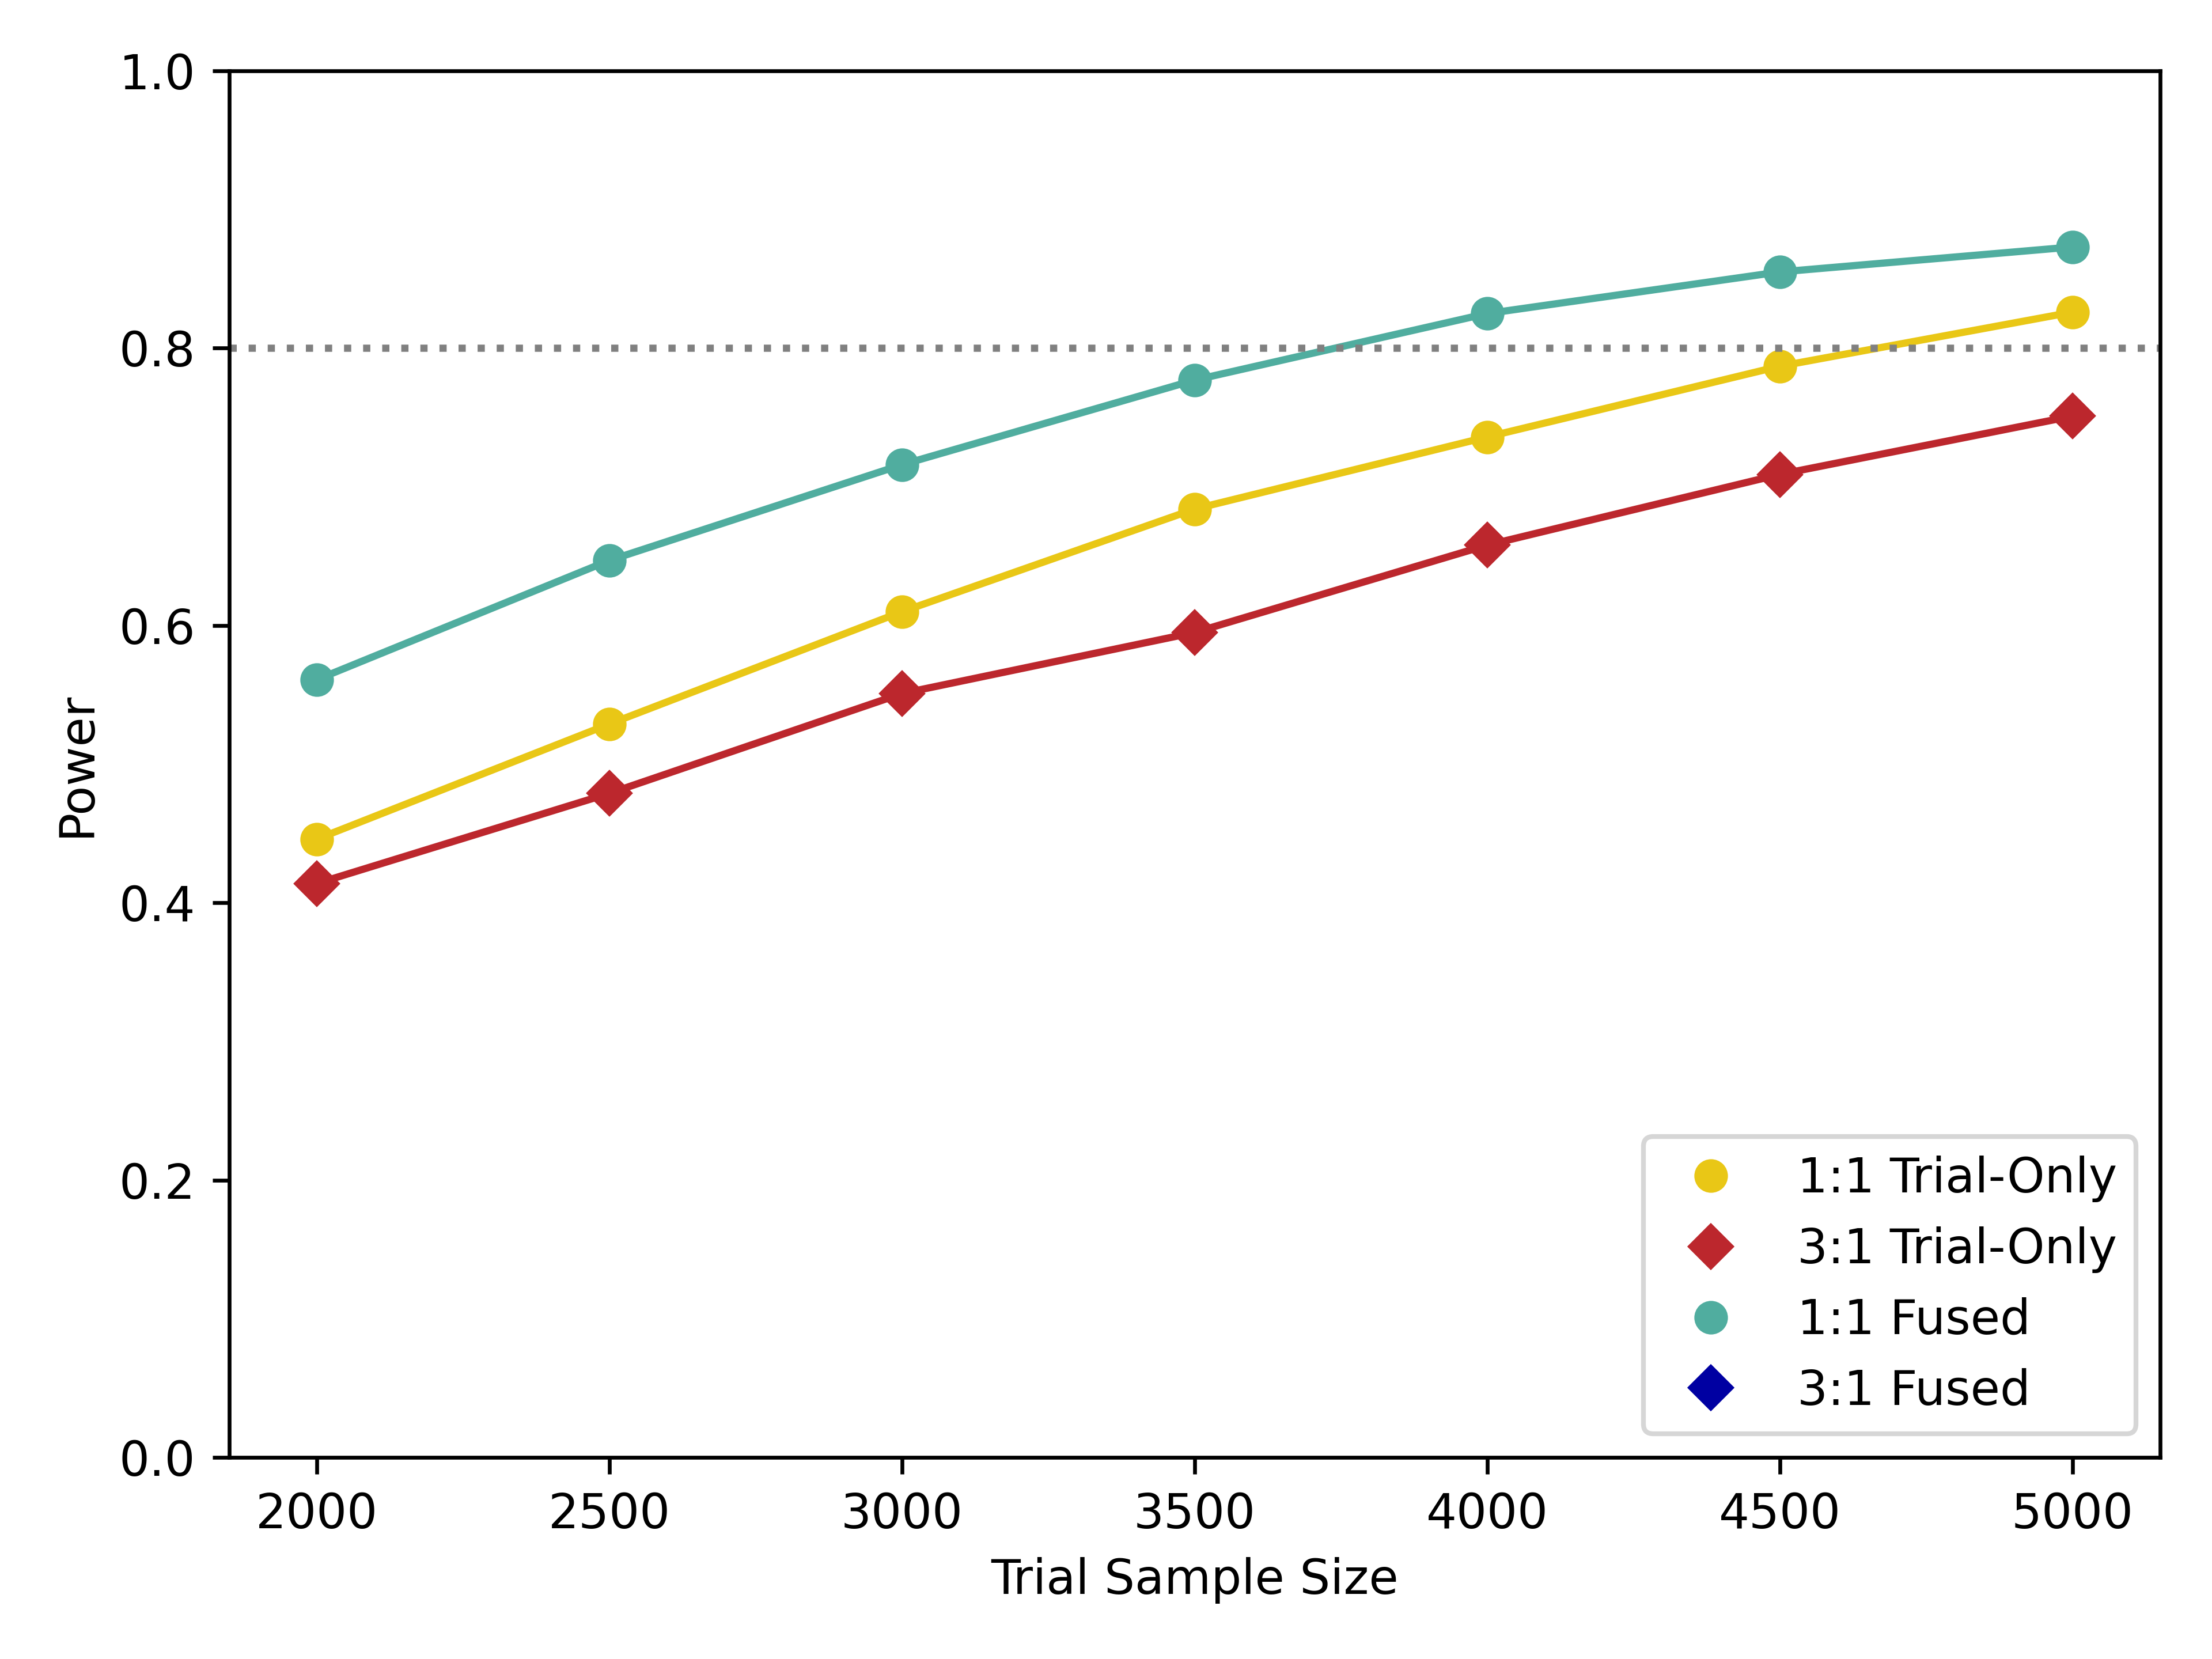
\includegraphics[width=0.9\linewidth]{images/power_trial-n_ser2.png}
	\end{center}
\end{frame}

\begin{frame}{Simulation -- Power by Trial Size\footnote[frame]{For an observational cohort of 5000}}
	\begin{center}
		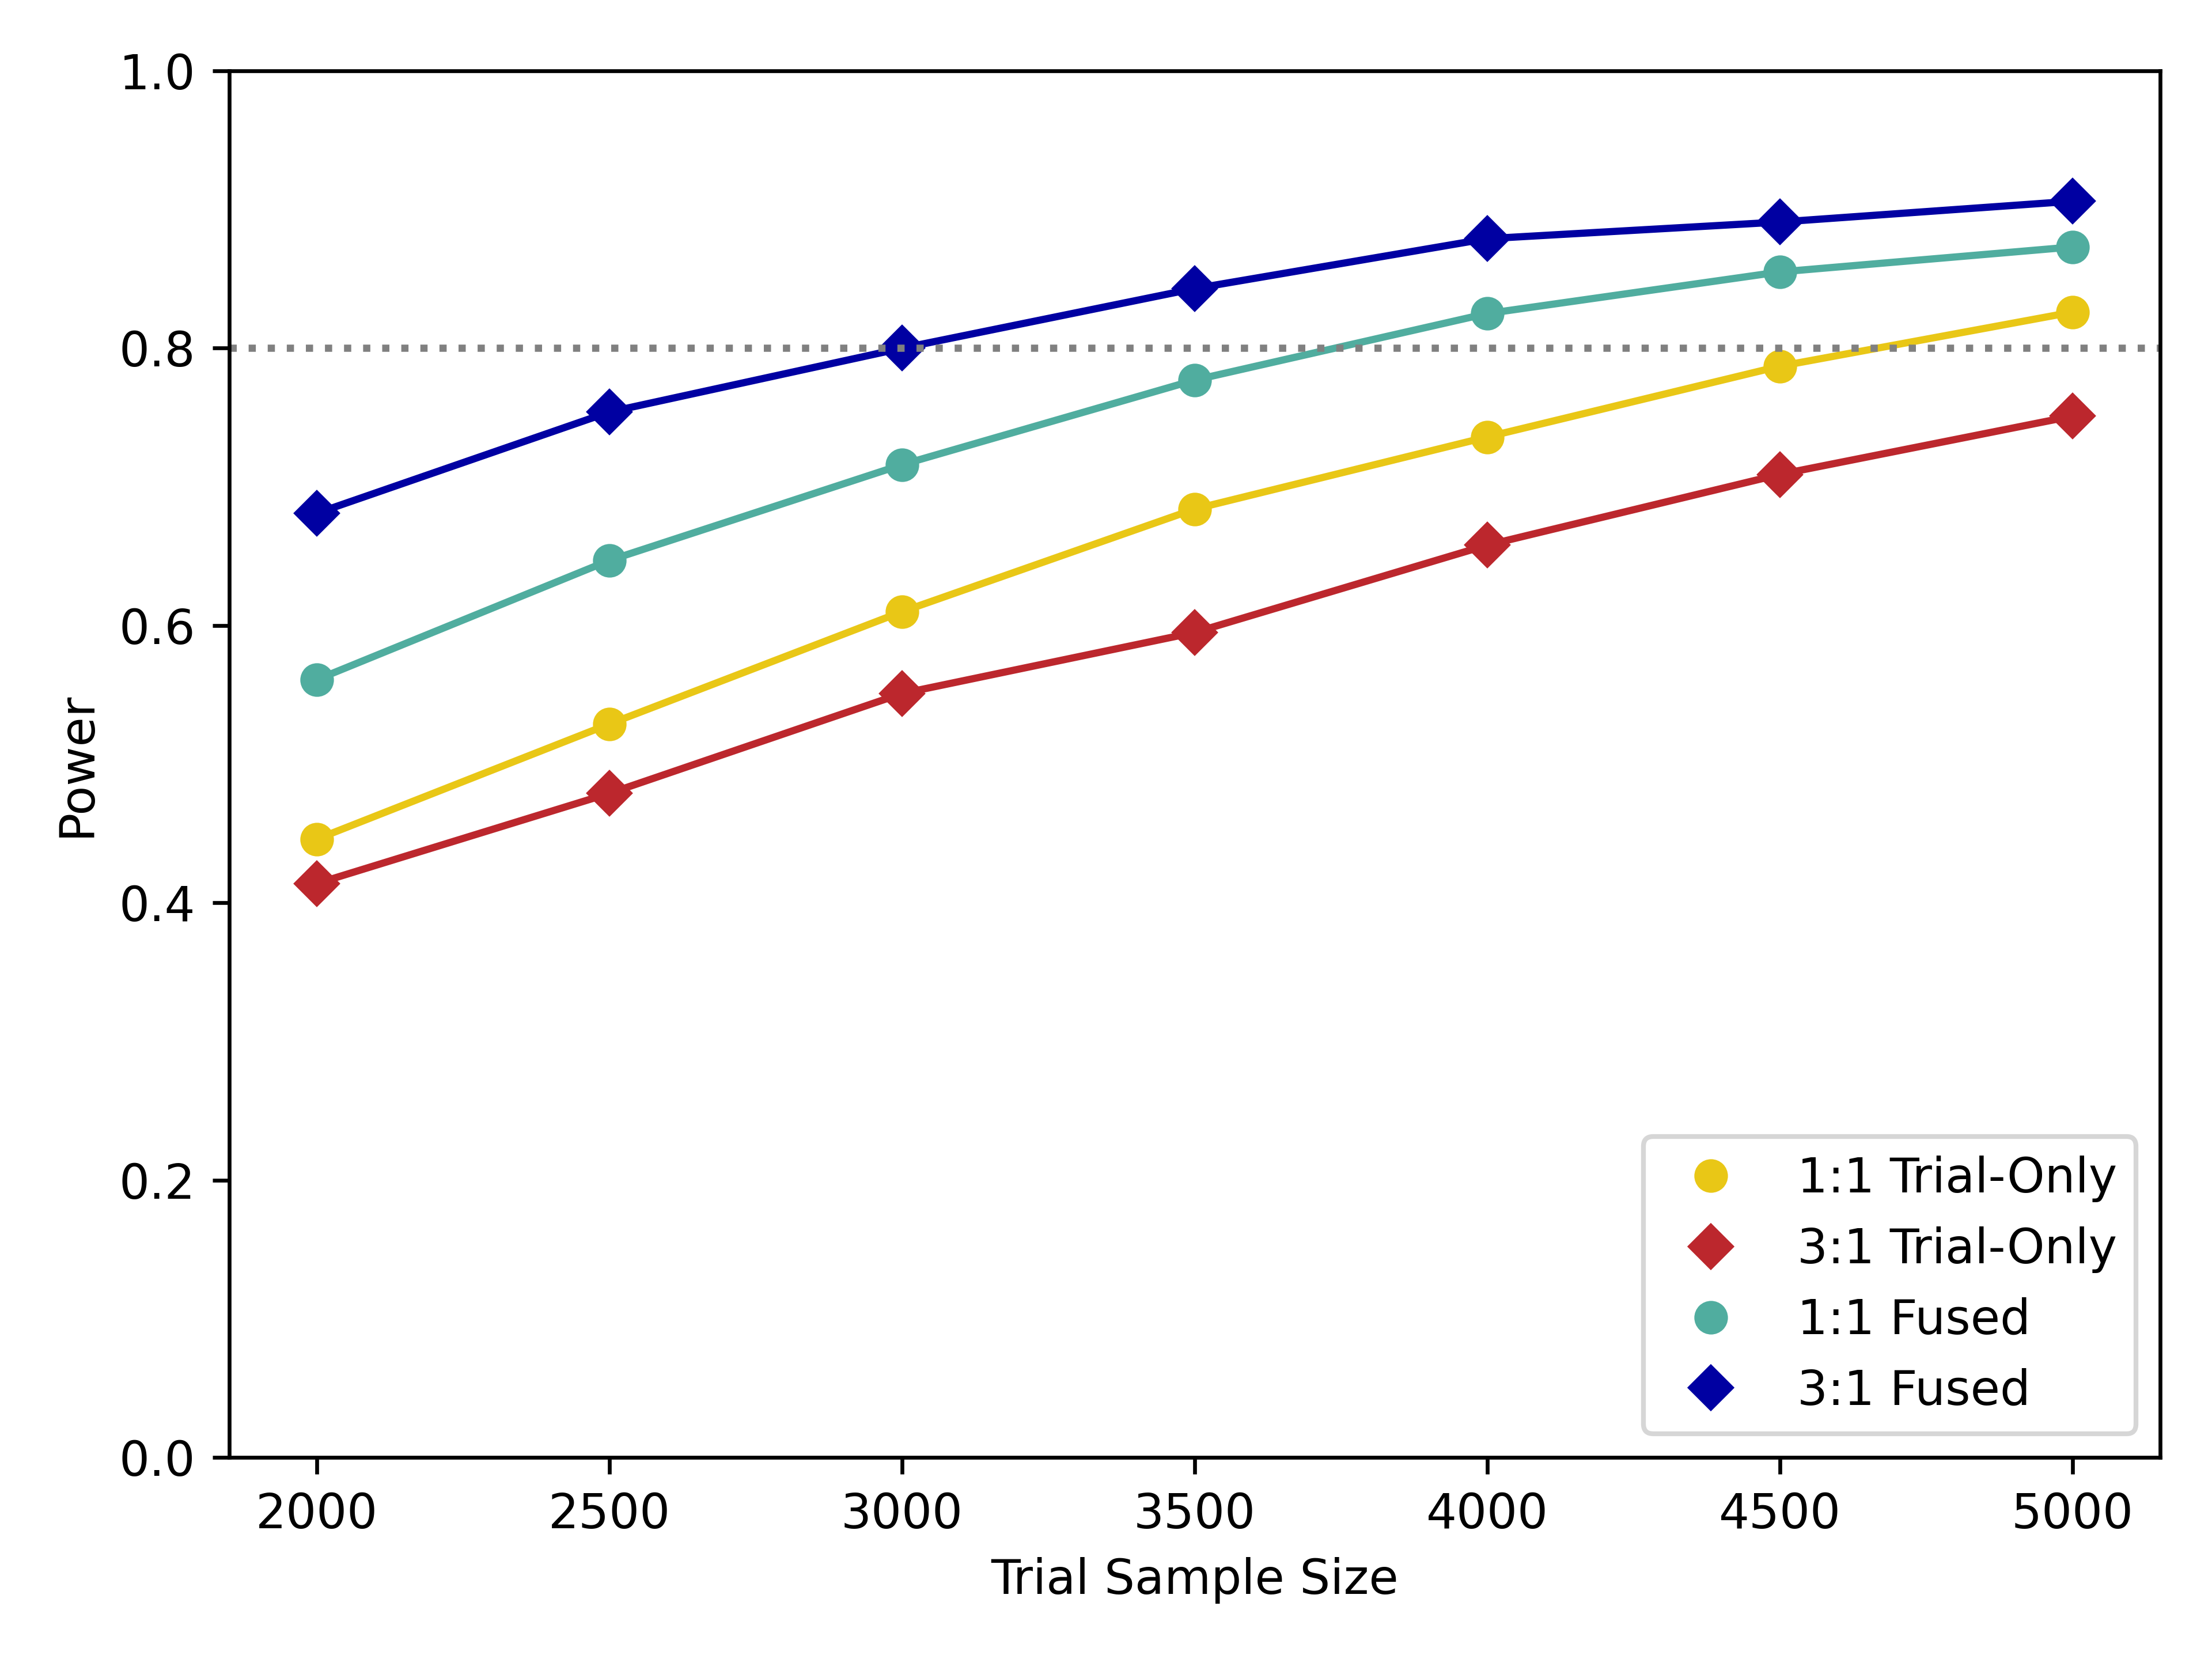
\includegraphics[width=0.9\linewidth]{images/power_trial-n_ser3.png}
	\end{center}
\end{frame}

\begin{frame}{Simulation -- Power by Cohort Size\footnote[frame]{For a trial of 2500}}
	\begin{center}
		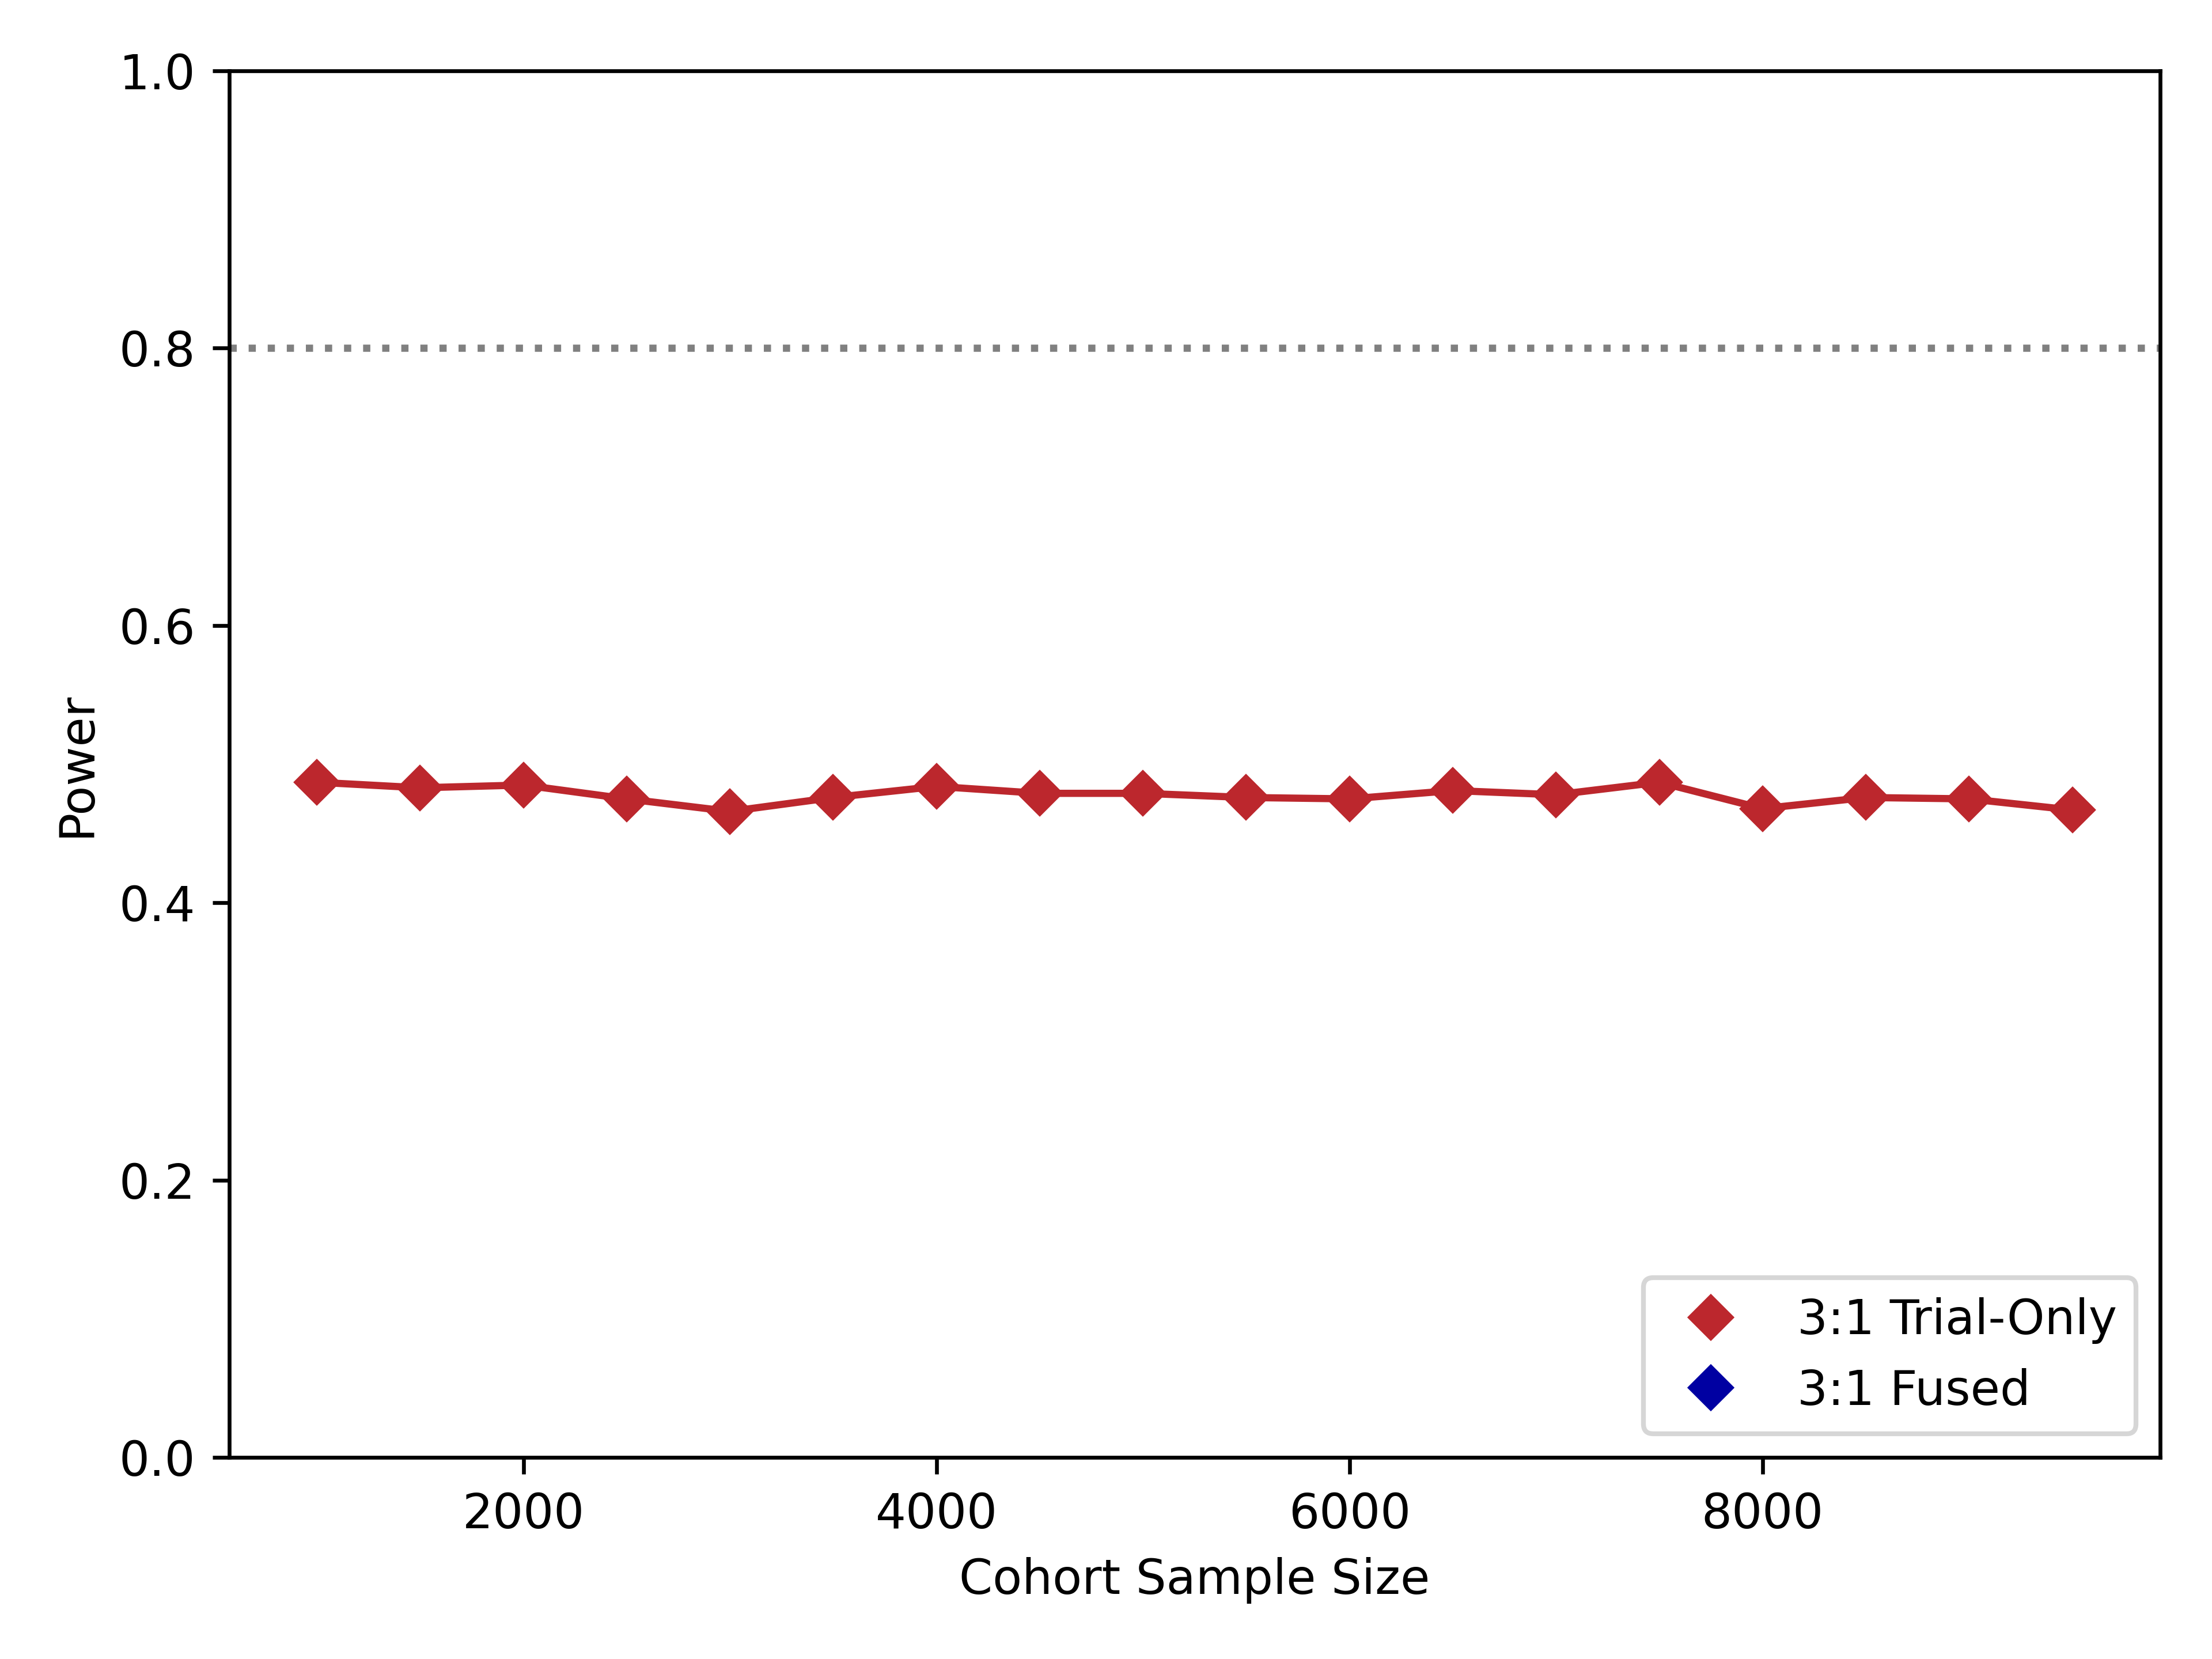
\includegraphics[width=0.9\linewidth]{images/power_obs-n_ser1.png}
	\end{center}
\end{frame}

\begin{frame}{Simulation -- Power by Cohort Size\footnote[frame]{For a trial of 2500}}
	\begin{center}
		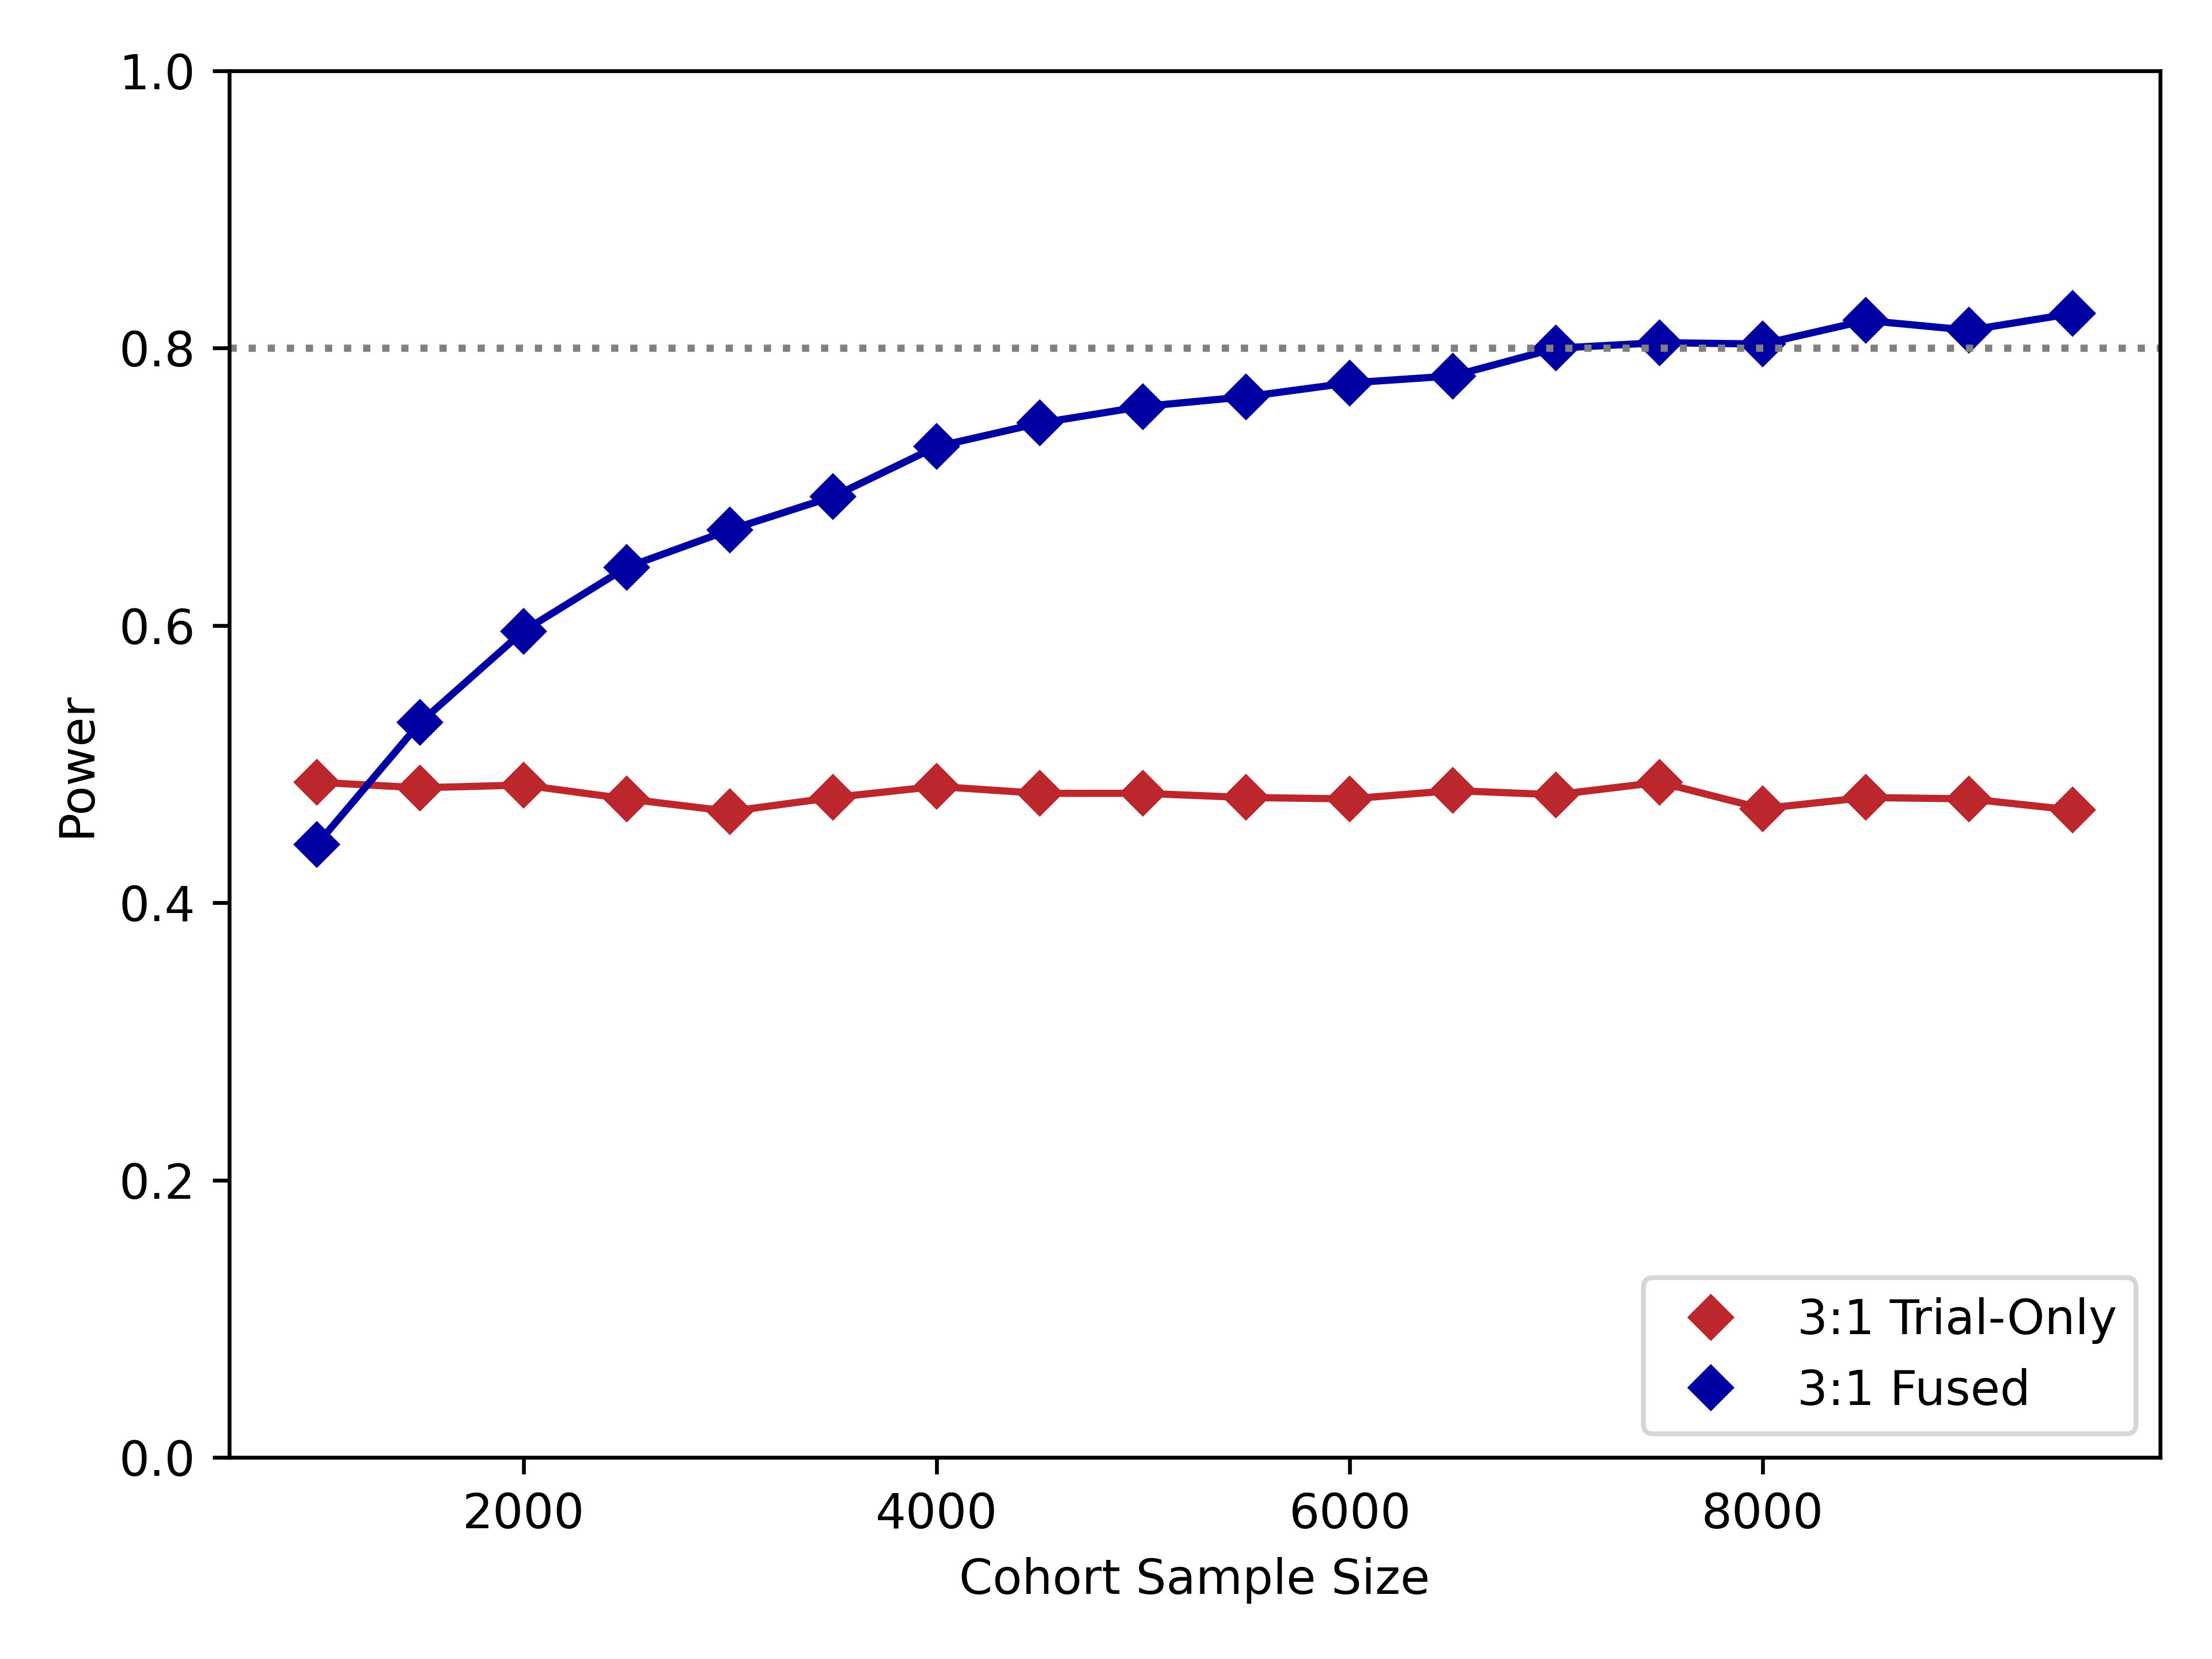
\includegraphics[width=0.9\linewidth]{images/power_obs-n_ser2.png}
	\end{center}
\end{frame}

\section{Conclusions}

\begin{frame}{Conclusions}
	Trials of LAI-ARV in infants face logistical challenges
	\begin{itemize}
		\item Low event rate under SOC
	\end{itemize}
	~\\
	Fusion estimator
	\begin{itemize}
		\item Improves power over standard trial design
		\item Tradeoffs
		\begin{itemize}
			\item Use of two models offers double robustness
			\item Less efficient than a g-computation fusion estimator when outcome model is correct
		\end{itemize}
	\end{itemize}
\end{frame}

\begin{frame}{Remaining Challenges}
	External data may introduce bias
	\begin{itemize}
		\item Violations of {\color{red}3.1} or {\color{red}3.2}
	\end{itemize}
	~\\
	Design-based mitigation strategies
	\begin{itemize}
		\item Randomize $S$
		\item Prospective observational cohort 
	\end{itemize}
	~\\
	Analysis-based mitigation strategies
	\begin{itemize}
		\item Randomization-Aware AIPW,\footnote[frame]{Gagnon-Bartsch et al. \textit{J Causal Inf} 2023; Karlsson et al. \textit{arXiv:2406.17971}} CV-TMLE\footnote[frame]{Dang et al. \textit{arXiv.2210.05802}}
	\end{itemize}
\end{frame}

\begin{frame}{Thank you}
	%\begin{center}
	%	{\Huge Questions?}
	%\end{center}
	%~\\~\\~\\
	\begin{center}
		\small
		\faEnvelope \quad pzivich@unc.edu \qquad \quad 
		\faGithub \quad pzivich \qquad \quad
		\faHashtag \quad pausalz@bsky.social
	\end{center}
\end{frame}

\section{Appendix}

\begin{frame}{Peformance Metrics}
	For trial of 2400 and cohort of 5000, operating characteristics were 
	\\~\\
	\begin{tabular}{lccccc}
		\hline
		& Bias  & ESE   & SER  & Coverage & Rejection \\ \cline{2-6} 
		Trial-Only    & 0.000 & 0.006 & 0.98 & 0.93     & 0.33      \\
		Naive Pooling & 0.006 & 0.003 & 1.00 & 0.38     & 0.29      \\
		AIPW          & 0.000 & 0.004 & 1.00 & 0.95     & 0.77      \\ \hline
	\end{tabular}
\end{frame}

\end{document}

